\chapter{Modelling Class Densities in a Frozen Feature Space}
\label{methodology}

\section{Proposed Architecture}

As shown in Figure~\ref{fig:architecture}, our CIL framework is built upon a simple yet structurally motivated decomposition: (i) a frozen feature extractor based on a visual foundation model, and (ii) a probabilistic classification layer that models each object category through an independent Gaussian distribution in the embedding space. Given an input image, the feature extractor maps it to a fixed high-dimensional representation. For each class, we maintain a class-conditional multivariate Gaussian characterized by its mean vector and covariance matrix, estimated incrementally from observed samples. Classification is performed according to the maximum likelihood principle, assigning the input to the class whose Gaussian model yields the highest likelihood under the stationary embedding representation. This modular separation between representation learning and statistical modeling enables incremental updates without backpropagation or parameter adaptation: adding a new class requires only estimating its distribution in the fixed feature space, while previously learned classes remain unaffected at the representation level.

\begin{figure}[htb]
	\centering
	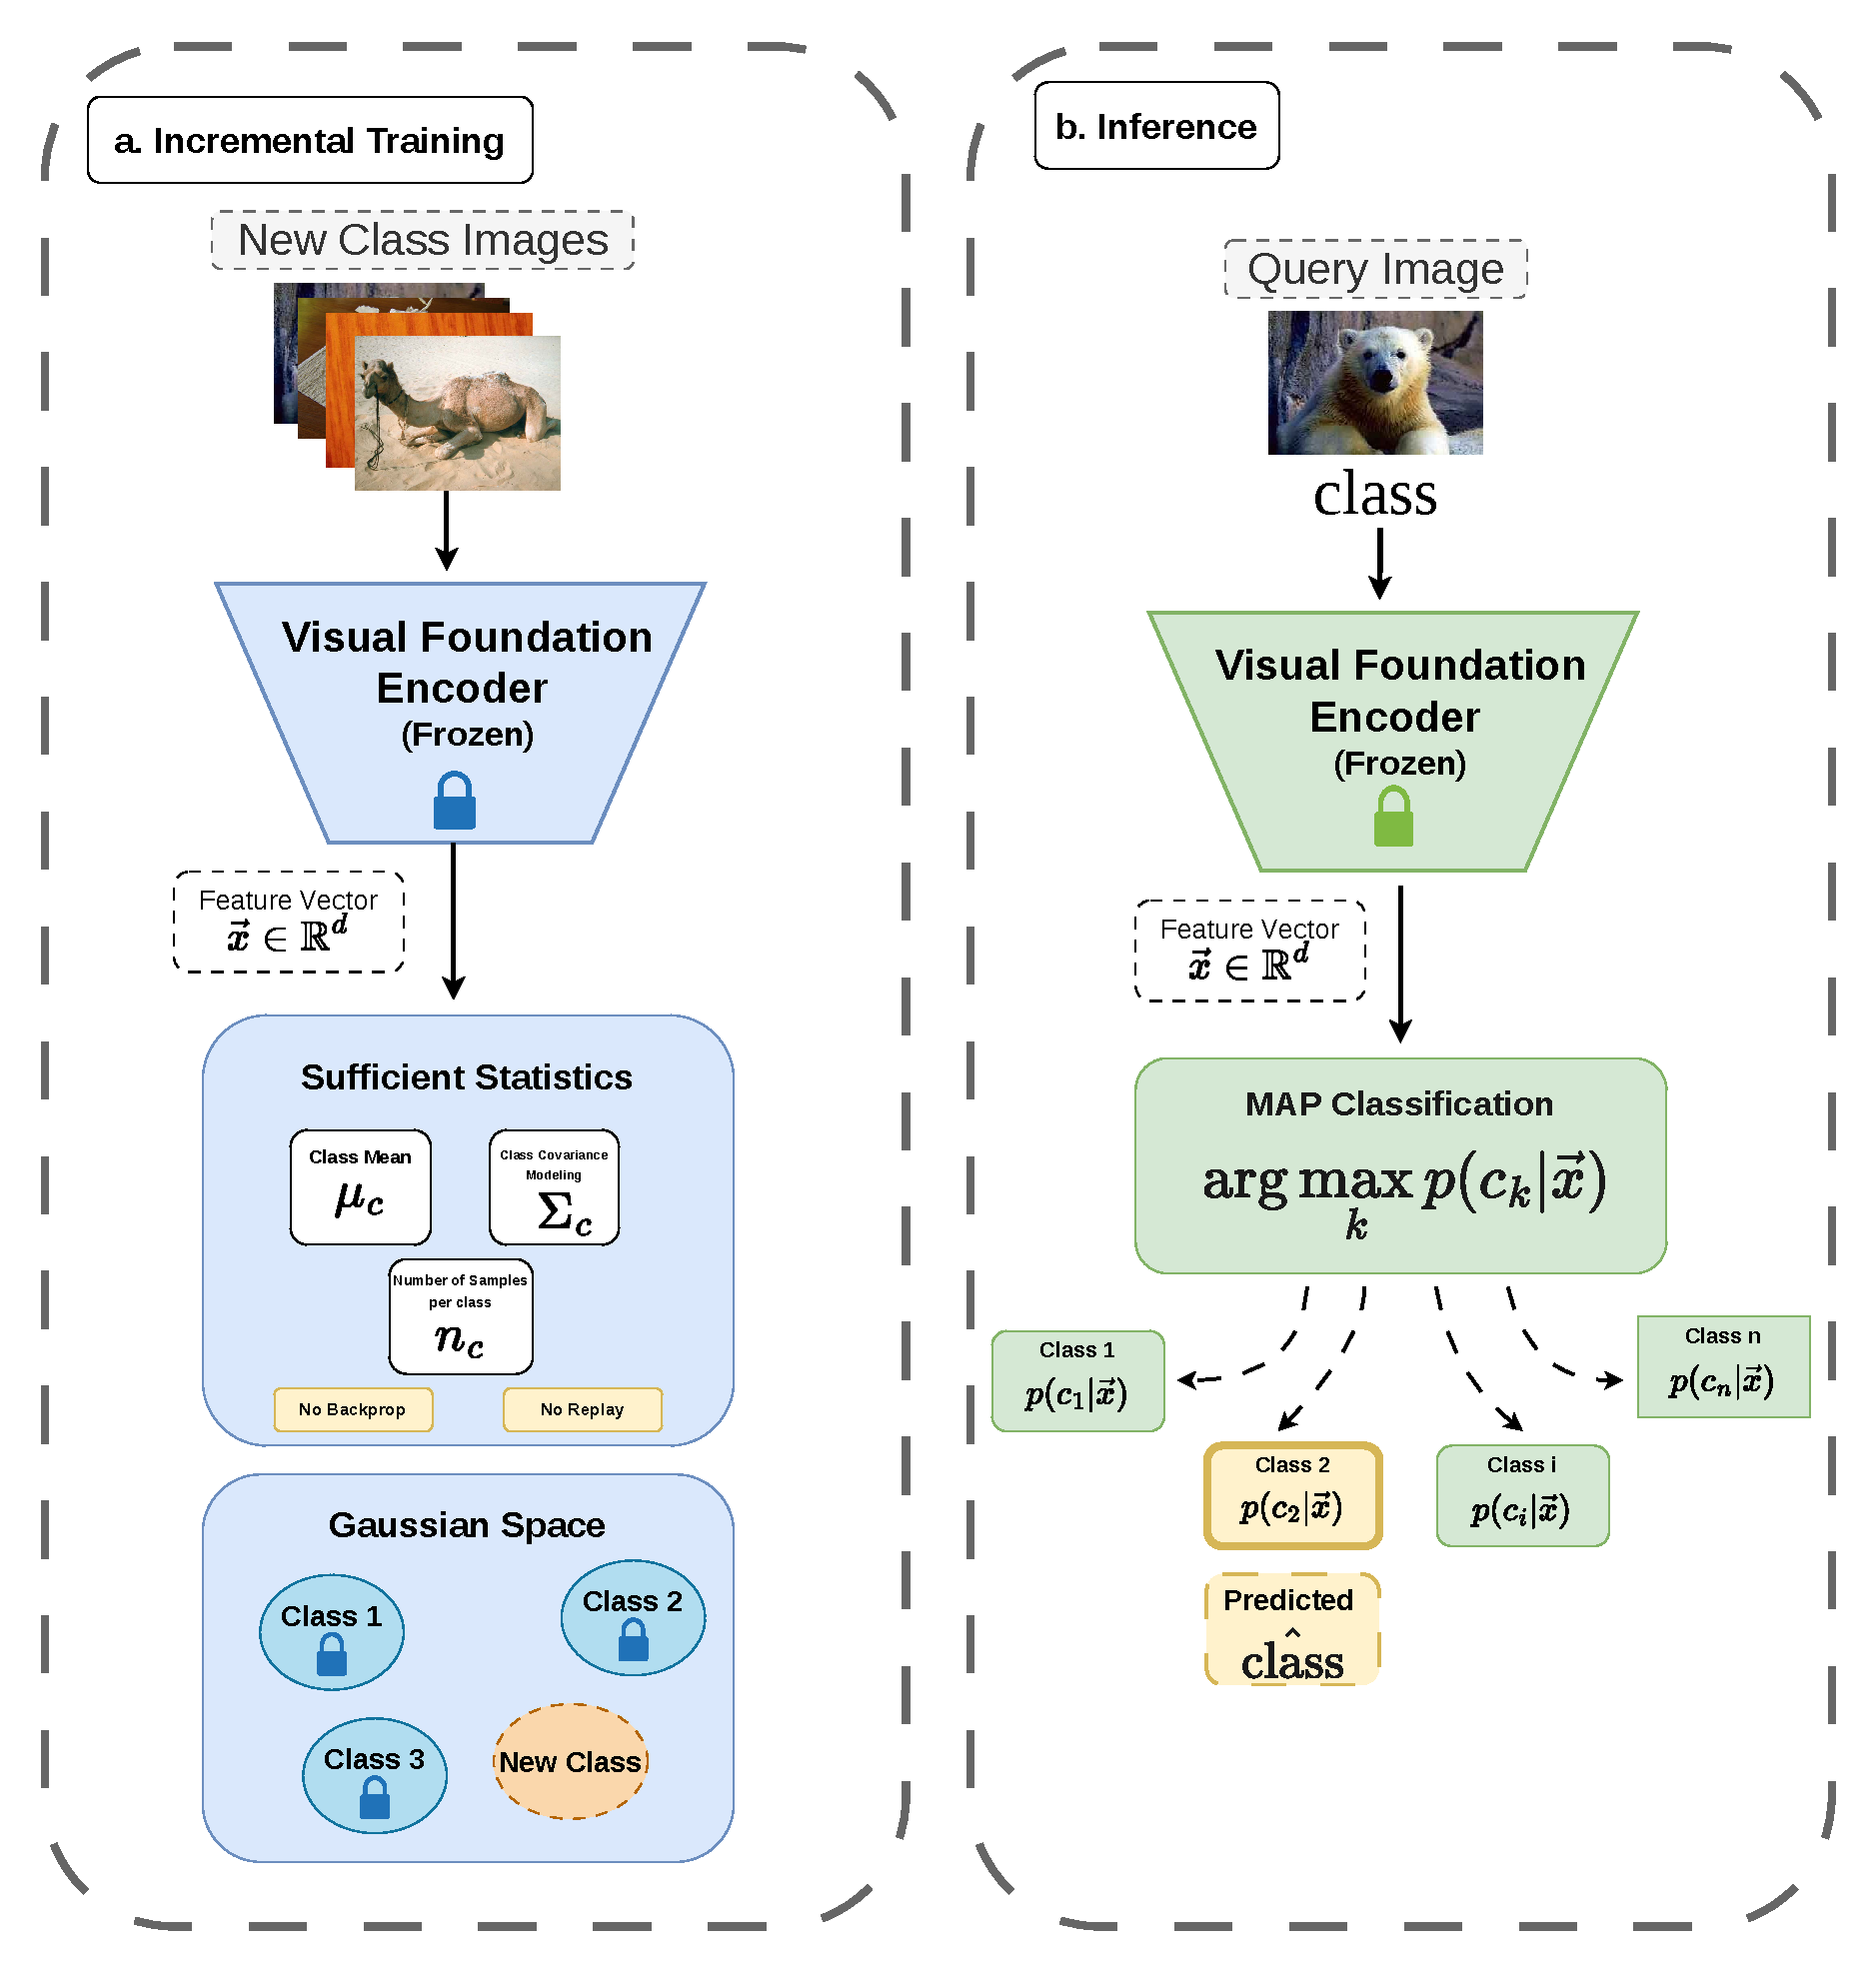
\includegraphics[width=0.6\textwidth]{imagenes/methodology/TMLR_block_diagram_approach.pdf}
	\caption{Overview of the proposed framework, reproduced from the peer-reviewed article that accompanies this thesis. A frozen foundation encoder maps each input image to a fixed embedding $\vec{x}\in\mathbb{R}^d$. Each class is represented by a Gaussian density (mean and covariance) that is updated incrementally without backpropagation. At inference, classification follows the MAP rule under the learned class-conditional densities. This diagram supersedes the general conceptual schematic used purely for narrative context in the Introduction (Figure~\ref{fig:intro_overview}), adding explicit detail on the recursive statistic-update mechanism shared by all covariance parameterisations introduced in Section~\ref{sec:covariance_estimation}.}
	\label{fig:architecture}
\end{figure}

\subsection{Likelihood-Based Classification}
\label{sec:method:classification}

Given an input image $x \in \mathcal{X}$, the frozen foundation model $\mathcal{F}$ produces a fixed-dimensional embedding
\begin{equation}
    \vec{x} = \mathcal{F}(x) \in \mathbb{R}^d
    \label{eq:feature_extractor}
\end{equation}
and all learning is performed directly in the stationary feature space $\mathbb{R}^d$. We adopt a generative modelling framework and assume class-conditional Gaussian feature distributions:
\begin{equation}
    p(\vec{x} \mid y = c) = \mathcal{N}(\vec{x} \mid \boldsymbol{\mu}_c,\, \boldsymbol{\Sigma}_c),
    \label{eq:class_gaussian}
\end{equation}
where $\boldsymbol{\mu}_c \in \mathbb{R}^d$ and $\boldsymbol{\Sigma}_c \succ 0$ are the class-specific mean and covariance matrix, estimated incrementally from observed samples. Classification is performed via Maximum A Posteriori (MAP) inference:
\begin{equation}
    \hat{y} = \arg\max_{c \in \mathcal{Y}} \left[ \log p(\vec{x} \mid y=c) + \log \pi_c \right],
    \label{eq:map}
\end{equation}
where $\pi_c = p(y=c)$ is the class prior. Under a uniform prior and the Gaussian density model, the decision rule is equivalent to the quadratic discriminant:
\begin{equation}
    \hat{y} = \arg\min_{c \in \mathcal{Y}} \left[ (\vec{x} - \boldsymbol{\mu}_c)^T \boldsymbol{\Sigma}_c^{-1} (\vec{x} - \boldsymbol{\mu}_c) + \log|\boldsymbol{\Sigma}_c| \right].
    \label{eq:qda}
\end{equation}
This quadratic decision function is the core of the proposed framework. The Mahalanobis term $(\vec{x}-\boldsymbol{\mu}_c)^T\boldsymbol{\Sigma}_c^{-1}(\vec{x}-\boldsymbol{\mu}_c)$ encodes the \emph{shape} of the class distribution while $\log|\boldsymbol{\Sigma}_c|$ encodes its \emph{volume}. The covariance parameterisations introduced in Section~\ref{sec:covariance_estimation} are specialisations of Equation~\eqref{eq:qda} that differ in the structure imposed on $\boldsymbol{\Sigma}_c$; the interplay between the shape and volume components is the central design axis of the covariance estimation study and is examined in detail in the analysis of results.

Adding a new class to the system requires only estimating the sufficient statistics $(\boldsymbol{\mu}_c, \boldsymbol{\Sigma}_c)$ in the fixed feature space; previously learned class statistics are never modified. This formulation therefore enables genuinely incremental updates without backpropagation, replay buffers, or exemplar storage.

\subsection{Datasets and Experimental Protocol}
We follow the standard Continual Learning (CL) protocol where the model learns a sequence of disjoint tasks and calculates the average accuracy and the forgetting. The four benchmarks used throughout this thesis are Split CIFAR-100, Split ImageNet-R, Split Caltech-256, and a heterogeneous Split Joint stream aggregating the three. The high-dimensional covariance estimators introduced in Section~\ref{sec:covariance_estimation} are stressed most heavily by the smallest of these per-class sample budgets, that of Split Caltech-256.

As mentioned, to quantify performance, SOTA works \cite{wang2022learning} utilize two standard metrics derived from the test accuracy scores: the average accuracy and the average forgetting.

With the architecture, benchmarks and evaluation metrics now in place, the remainder of this chapter follows a single, consistent narrative arc that Chapter~\ref{ch:results} mirrors section by section: it opens with the covariance-estimation methodology and its mixture-of-Gaussians extensions, then introduces the incremental class-inclusion protocol that stresses the growing decision surface, and closes with the sensitivity of the framework to the choice of upstream backbone. The feature-space characterization tools that these methodological choices rely on---the probabilistic confidence and calibration metrics, the inter-class pairwise Bhattacharyya and Euclidean distances, the spectral structure of the embedding space, and the statistical validation of the Gaussianity assumption on which the whole framework rests---are developed together in Chapter~\ref{ch:gaussian_space}.

\section{Covariance Estimation}
\label{sec:covariance_estimation}

Due to the high dimensionality of the extracted feature ($\vec{x}\in \mathbb{R}^d$), the empirical sample covariance matrix (SCM) is a poor estimator for each class: its eigenvalues are biased, and the matrix is singular whenever $n_c < d$. In our setting $d = 768$ while $n_c$ ranges from approximately $40$ to $400$ depending on the benchmark, so the matrix always has at most $n_c - 1$ non-zero eigenvalues out of $d = 768$, leaving $d - (n_c - 1)$ eigenvalues that are structurally zero before any regularisation is applied.
The Gaussian modelling assumption that motivates the covariance-based classifiers introduced below is formally validated later in Section~\ref{sec:method:gaussianity_main}; here we focus on how to obtain a well-conditioned covariance estimate under that assumption. Our benchmarks are tested using different covariance estimation methods:

\subsection{Diagonal Covariances}
In this configuration, we assume that the features within each class $c$ are independent, leading to a diagonal covariance matrix $\boldsymbol{\Sigma}_c = \text{diag}(\sigma_{c,1}^2, \sigma_{c,2}^2, \dots, \sigma_{c,d}^2)$. This simplification significantly reduces the number of parameters to estimate from $O(d^2)$ to $O(d)$, which is particularly advantageous when the dimensionality $d = 768$ is large relative to the number of samples per class. For each class $c \in \{1, \dots, C\}$, the mean vector $\boldsymbol{\mu}_c$ and the diagonal elements of $\boldsymbol{\Sigma}_c$ are computed as:

\begin{equation}
	\boldsymbol{\mu}_c = \frac{1}{n_c} \sum_{i=1}^{n_c} \vec{x}_i, \quad \sigma_{c,j}^2 = \frac{1}{n_c-1} \sum_{i=1}^{n_c} (x_{i,j} - \mu_{c,j})^2 + \epsilon
\end{equation}
where $\epsilon = 10^{-6}$ is a small constant added to ensure numerical stability and strictly positive variances. The log-likelihood of a test sample $\vec{x}$ belonging to class $c$ is determined by the discriminant function:

\begin{equation}
	g_c(\vec{x}) = \ln P(\vec{x}|c) + \ln P(c)
\end{equation}

Under the assumption of a uniform prior $P(c)$ and Gaussian distribution, this simplifies to:

\begin{equation}
	g_c(\vec{x}) = -\frac{1}{2} \sum_{j=1}^{d} \left( \ln(2\pi\sigma_{c,j}^2) + \frac{(x_j - \mu_{c,j})^2}{\sigma_{c,j}^2} \right)
\end{equation}


\subsection{Full Covariances}
\label{sec:method:full_cov}

To account for the dependencies between different dimensions of the feature vector, we estimate a full covariance matrix $\boldsymbol{\Sigma}_c \in \mathbb{R}^{d \times d}$ for each class $c$. While this provides a richer representation of the class distribution, the estimation of $d^2$ parameters is prone to ill-conditioning when the number of samples $n_c$ is limited.The mean vector $\boldsymbol{\mu}_c$ and the empirical covariance $\boldsymbol{\Sigma}_c$ are calculated as:

\begin{equation}
	\boldsymbol{\mu}_c = \frac{1}{n_c} \sum_{i=1}^{n_c} \vec{x}_i, \quad \boldsymbol{\Sigma}_c = \frac{1}{n_c - 1} \sum_{i=1}^{n_c} (\vec{x}_i - \boldsymbol{\mu}_c)(\vec{x}_i - \boldsymbol{\mu}_c)^T
\end{equation}

To ensure that the matrix is invertible and to improve numerical stability, a regularization is applied by adding a small identity term to the diagonal: $\hat{\boldsymbol{\Sigma}}_c = \boldsymbol{\Sigma}_c + \epsilon I$, with $\epsilon = 10^{-6}$.

For obtaining the precision matrix $Q_c$ (the inverse of the covariance matrix $\hat{\boldsymbol{\Sigma}}_c$), an approach based on Cholesky decompositions is used. The covariance $\hat{\boldsymbol{\Sigma}}_c$ is decomposed as
\begin{equation}
	\hat{\boldsymbol{\Sigma}}_c = C_c C_c^T, \qquad C_c L_c = I,
	\label{eq:cholesky_decomp}
\end{equation}
with $C_c$ lower triangular and $I$ the identity, so that $L_c = C_c^{-1}$ is the Cholesky factor of the precision matrix $Q_c = L_c^T L_c$.

Then, the squared Mahalanobis distance and the log-determinant are computed from $\boldsymbol{\mu}_c$ and $L_c$ as:

\begin{equation}
	d_M(\vec{x}, \boldsymbol{\mu}_c, L_c) = (\vec{x} L_c - \boldsymbol{\mu}_c L_c)^T (\vec{x} L_c - \boldsymbol{\mu}_c L_c)
	\label{eq:cholesky_mahalanobis}
\end{equation}

\begin{equation}
	\ln |\hat{\boldsymbol{\Sigma}}_c| = 2 \sum_{i=1}^{d}{\ln(L_{c \, i,i})}
	\label{eq:cholesky_logdet}
\end{equation}

\subsection{Hybrid Covariance}
\label{sec:method:hybrid_cov}

The hybrid covariance estimator decouples the squared Mahalanobis distance from its associated normalisation constant. For each class $c$, the full covariance matrix $\hat{\boldsymbol{\Sigma}}_c$ is estimated and regularised exactly as in Section~\ref{sec:method:full_cov}, and the squared Mahalanobis distance $d_M(\vec{x}, \mu_c, L_c)$ is computed using the same Cholesky-based procedure of Equations~\eqref{eq:cholesky_decomp}--\eqref{eq:cholesky_mahalanobis}, so that the \emph{shape} of the discriminant retains the full off-diagonal structure of the empirical covariance. However, the log-determinant term---which represents the \emph{volume} of the distribution---is computed using only the diagonal elements (variances) of the covariance matrix:
\begin{equation}
	\ln |\hat{\boldsymbol{\Sigma}}_c|_{\text{diag}} = \sum_{j=1}^{d} \ln(\sigma_{c,j}^2),
	\label{eq:hybrid_logdet}
\end{equation}
where $\sigma_{c,j}^2$ denotes the $j$-th diagonal entry of $\hat{\boldsymbol{\Sigma}}_c$. The resulting discriminant function is defined as:
\begin{equation}
	g_c(\vec{x}) = -\frac{1}{2} \left( d \ln(2\pi) + \sum_{j=1}^{d} \ln(\sigma_{c,j}^2) + d_M(\vec{x}, \boldsymbol{\mu}_c, L_c) \right).
	\label{eq:hybrid_discriminant}
\end{equation}

This formulation avoids the numerical issues that arise when near-zero eigenvalues of $\hat{\boldsymbol{\Sigma}}_c$ artificially inflate or destabilise the exact log-determinant, at the cost of using a diagonal approximation for the volume term only.

\subsection{OAS Covariance}
\label{sec:method:oas}

Oracle Approximating Shrinkage (OAS) is a shrinkage technique that computes an structurally optimized covariance matrix by finding an optimal compromise between the sample covariance matrix and a structured target (the identity matrix scaled by the average trace).The OAS estimator provides a more accurate estimation of the covariance $\boldsymbol{\Sigma}_c$ by minimizing the Mean Squared Error (MSE) under the assumption of Gaussianity. The estimated covariance is defined as:

\begin{equation}
	\hat{\boldsymbol{\Sigma}}_{\text{OAS}, c} = (1 - \rho_c) \hat{\boldsymbol{\Sigma}}_{\text{SCM}, c} + \rho_c \hat{F}_c
\end{equation}
where $\rho_c$ is the shrinkage coefficient calculated specifically for class $c$, $\hat{\boldsymbol{\Sigma}}_{\text{SCM}, c}$ is the sample covariance matrix, and $\hat{F}_c = \frac{\text{tr}(\hat{\boldsymbol{\Sigma}}_{\text{SCM}, c})}{d} I$ is the shrinkage target.In our implementation, we compute the precision matrix $\Psi_c = \hat{\boldsymbol{\Sigma}}_{\text{OAS}, c}^{-1}$ directly via the OAS algorithm. This precision matrix is then used to calculate the Mahalanobis distance in the log-likelihood discriminant function:

\begin{equation}
	g_c(\vec{x}) = \ln A_c - \frac{1}{2} (\vec{x} - \boldsymbol{\mu}_c)^T \Psi_c (\vec{x} - \boldsymbol{\mu}_c)
\end{equation}

where $\ln A_c$ is the normalization constant derived from the log-determinant of the OAS-estimated covariance matrix, evaluated numerically via the stable log-determinant of the eigendecomposition. This approach ensures that the model captures class-specific correlations while remaining robust to the ``curse of dimensionality.''

\subsection{Ledoit-Wolff}
\label{sec:method:ledoitwolf}

The Ledoit-Wolf Diagonal Anchor estimator addresses the instability of the sample covariance matrix $S$ by shrinking it toward a target matrix $T$.

The selection of a target matrix $T$ represents a prior assumption regarding the feature distribution. Both methods stabilize the estimator by pulling the noisy off-diagonal elements of the sample covariance matrix $S$ toward zero, but they differ in how they treat the diagonal elements (the variances).

\subsubsection{Diagonal Target}
The diagonal anchor is defined as $T_{\text{diag}} = \text{diag}(s_{11}, s_{22}, \dots, s_{dd})$. This approach assumes that the features are independent but allows for heteroscedasticity, meaning each dimension can have a different variance. Shrinkage toward this target preserves the scale of each individual feature as observed in the sample data while suppressing only the correlations. This is particularly useful when certain dimensions of the DINOv2 embeddings are naturally more informative or volatile than others.

\subsubsection{Identity Target}The identity anchor is more restrictive, defined as $T_{\text{ident}} = \mu I$, where $\mu = \frac{1}{d} \text{tr}(S)$ is the average variance across all dimensions. This target assumes that the features are not only independent but also share a common variance (homoscedasticity). The resulting distribution is spherical. Because the embeddings used in this work are L2-normalized, the variances across dimensions tend to be similar, making the identity anchor a highly robust regularizer that prevents any single dimension from disproportionately influencing the distance metric.

\subsubsection{Structural Summary}The fundamental difference between these two estimators lies in the flexibility of the variance components:

\begin{itemize}
	\item \textbf{Diagonal Anchor:} $\hat{\Sigma}_{ij} = (1-\gamma)s_{ij}$ for $i \neq j$, and $\hat{\Sigma}_{ii} = s_{ii}$. It yields an axis-aligned ellipsoidal distribution.
	\item \textbf{Identity Anchor:} $\hat{\Sigma}_{ij} = (1-\gamma)s_{ij}$ for $i \neq j$, and $\hat{\Sigma}_{ii} = (1-\gamma)s_{ii} + \gamma \mu$. It yields a distribution that is pulled toward a perfectly spherical geometry.
\end{itemize}

\subsection{Shared Covariance}
\label{subsec:shared_cov_original}

The Shared Covariance framework assumes that the internal noise or feature variability is homoscedastic across all classes. In this paradigm, all classes share a single covariance matrix $\boldsymbol{\Sigma}$, which captures the global structure of the feature space.

A key aspect of this framework in the continual learning setting is that $\boldsymbol{\Sigma}$ is re-estimated at the end of each task $t$ using only the classes observed so far, $\mathcal{C}_t = \{1, \dots, C_t\}$.

\section{Mixture of Gaussians}

In order to capture potential multi-modality within the feature space of a single class, we employ Gaussian Mixture Models (GMM). We implemented the following models using the previously defined diagonal, full and hybrid covariances approaches.

\subsection{Mixture of 2 Gaussians}

Forcing each class to be defined as a GMM with $K=2$ components, each class $c$ can be modeled by a probability density function:

\begin{equation}
	p(\vec{x}|c) = \sum_{k=1}^{K} \pi_{c,k} \mathcal{N}(\vec{x} | \boldsymbol{\mu}_{c,k}, \boldsymbol{\Sigma}_{c,k})
\end{equation}

where $\pi_{c,k}$ represents the mixing weight of the $k$-th component for class $c$, subject to $\sum \pi_{c,k} = 1$. In this specific variant, the covariance matrices $\boldsymbol{\Sigma}_{c,k}$ are restricted to be diagonal to maintain computational efficiency and prevent over-fitting in the high-dimensional DINOv2 space.The parameters $\{\pi_{c,k}, \boldsymbol{\mu}_{c,k}, \boldsymbol{\Sigma}_{c,k}\}$ are estimated using the Expectation-Maximization (EM) algorithm. To ensure numerical stability, a small constant $\epsilon = 10^{-5}$ is added to the diagonal of each covariance matrix. The log-likelihood for a test sample $\vec{x}$ is calculated using the \textit{LogSumExp} operator to avoid underflow:

\begin{equation}
	\ln p(\vec{x}|c) = \text{lnaddexp} \left( \ln(\pi_{c,1} \mathcal{N}(\vec{x} | \boldsymbol{\mu}_{c,1}, \boldsymbol{\Sigma}_{c,1})), \ln(\pi_{c,2} \mathcal{N}(\vec{x} | \boldsymbol{\mu}_{c,2}, \boldsymbol{\Sigma}_{c,2})) \right)
\end{equation}

In the implementation, this is expanded as:

\begin{equation}
	\ln p(\vec{x}|c) = \ln \left( \exp( \ln \pi_{c,1} + \ln A_{c,1} - \frac{1}{2} d_{M,1} ) + \exp( \ln \pi_{c,2} + \ln A_{c,2} - \frac{1}{2} d_{M,2} ) \right)
\end{equation}

where $d_{M,k}$ is the diagonal Mahalanobis distance to the $k$-th component and $\ln A_{c,k}$ is the normalization constant. This approach allows the model to better represent classes that may contain significantly different visual sub-types or clusters within the latent embedding space.


\subsection{Mixture of up-to-4 Gaussians}

To adapt to the varying complexity of different classes within the different datasets, we implement a flexible Gaussian Mixture Model where the number of components $K_c$ for each class $c$ is not fixed. Instead, the model selects the most appropriate number of components $K_c \in \{1, 2, 3, 4\}$ by minimizing the Bayesian Information Criterion (BIC).The BIC is defined as:

\begin{equation}
	\text{BIC} = \ln(n)k - 2\ln(\hat{L})
	\label{eq:bic_mog4}
\end{equation}

where $n$ is the number of samples in the class, $k$ is the number of free parameters to be estimated, and $\hat{L}$ is the maximized value of the likelihood function. By using diagonal covariance matrices, the number of parameters per component is kept low ($2d + 1$), allowing the selection process to favor multi-modal distributions only when the increase in likelihood justifies the additional parameters. For each component $k$ in class $c$, the diagonal covariance $\boldsymbol{\Sigma}_{c,k} = \text{diag}(\sigma_{c,k,1}^2, \dots, \sigma_{c,k,d}^2)$ is regularized with $\epsilon = 10^{-6}$. The classification of a test sample $\vec{x}$ involves calculating the weighted log-likelihood across all active classes:

\begin{equation}
	\ln p(\vec{x}|c) = \text{LSE}_{k=1}^{K_c} \left( \ln \pi_{c,k} - \frac{1}{2} \left( \sum_{j=1}^{d} \ln(2\pi\sigma_{c,k,j}^2) + \sum_{j=1}^{d} \frac{(x_j - \mu_{c,k,j})^2}{\sigma_{c,k,j}^2} \right) \right)
\end{equation}

where $\text{LSE}$ denotes the LogSumExp operator. This methodology allows for a more granular representation of class distributions—using a single Gaussian for simple, compact classes and up to four Gaussians for classes with high intra-class variance or distinct visual sub-clusters—while preserving the numerical efficiency of diagonal estimators.

\section{Incremental Class Inclusion}
\label{sec:method:incremental}

Having defined the full family of covariance estimators in Section~\ref{sec:covariance_estimation}, we design a class-incremental evaluation protocol to systematically assess how each closed-form estimator scales as the overall classification task grows in complexity. Rather than measuring conventional catastrophic forgetting—given that each class-conditional Gaussian is estimated independently and frozen upon initialization—this incremental class inclusion experiment isolates the impact of a progressively hardening decision surface on classification performance. By sequentially expanding the set of active classes and tracking the evolution of average accuracy over the growing pool of target categories, we can observe how the physical expansion of the label space translates into geometric crowding within the underlying feature space. This experimental design directly bridges empirical performance degradation with the architectural geometry of the learned representations, paving the way to quantify how the introduction of new class-conditional distributions compresses the margins between prototype boundaries and intensifies pairwise class confusion.


\section{Backbones Comparison}
\label{sec:method:backbones}

Throughout this work, DINOv2 \cite{oquab2024dinov} is used as the default backbone feature extractor for the Gaussian-based classifiers because of its self-supervised training regime and the strong empirical evidence of approximately Gaussian, well-conditioned class-conditional distributions presented in Section~\ref{sec:method:gaussianity_main}. However, the proposed framework is agnostic to the specific feature extractor used: any frozen encoder that produces fixed-dimensional embeddings can plug in unchanged into the downstream Gaussian classifier. To quantify the dependence of the framework on the choice of backbone, we further analyse the impact of the backbone architecture by re-running the Diag-Cov and Full-Cov variants using two supervised Vision Transformers from the \texttt{timm} library \cite{rw2019timm}: \textbf{ViT-base/16} (ViT-b, $d=768$) and \textbf{ViT-medium/16} (ViT-m, $d=512$), both pre-trained on ImageNet-21k \cite{imagenet21k}. The covariance estimation, hyper-parameters and evaluation protocol are kept identical across backbones to isolate the effect of the upstream representation; the results are reported in Section~\ref{sec:backbone_results}.

This concludes the description of the proposed methodology: the frozen-backbone Gaussian architecture, the covariance-estimation family and its mixture-of-Gaussians extensions, the incremental class-inclusion protocol, and the backbone-sensitivity ablation. Chapter~\ref{ch:gaussian_space} develops, in a single consolidated treatment, the mathematical and statistical tools---spectral analysis, Gaussianity testing, inter-class separability, and confidence calibration---used to characterize the feature space these methods operate on, before Chapter~\ref{ch:results} reports and interprets the resulting empirical evidence.
